\documentclass[a4paper,10pt]{scrartcl}

% Hier die Nummer des Blatts und Autoren angeben.
\newcommand{\blatt}{1}
\newcommand{\autor}{Jim Martens}

\usepackage{hci}
\usepackage[utf8]{inputenc}
\usepackage{float}

\begin{document}
% Seitenkopf mit Informationen
\kopf
\renewcommand{\figurename}{Figure}

\aufgabe{1}

In dem Thought Paper "`The Ultimate Display"' von Ivan E. Sutherland geht es um ein zukünftiges Display, das sich um den Menschen herum erstreckt. Der Mensch steht in dem Display und das Display kann Materie kontrollieren innerhalb dieses Raumes. So könnte es Stühle erzeugen, Objekte verschieben und eben diese auch wieder auflösen. Ein Unfall oder Mord in dem Display wären defacto Realität, denn Kugeln in dem Display wären tödlich.

Der Mensch könnte mit der vom Display kontrollierten Materie interagieren und sich beispielsweise auf einen Stuhl setzen.

In der Hinleitung zu diesem Ultimate Display erwähnt Sutherland die (zum Zeitpunkt des Erscheinens des Papers) aktuellen Displays und zeigt ihre Schwachstellen auf. Ferner geht er auf technische Erfordernisse der Mensch-Computer-Interaktion ein und erwähnt Mäuse, Tastaturen, Joysticks, Tablets (nicht die heutigen) sowie die menschliche Stimme.

\aufgabe{2.1}

Das Gerät muss folgende Anforderungen erfüllen, um den Inuit von Grönland bei der Navigation mit Kanus an der Küste zu helfen:

\begin{itemize}
	\item kann Standort bestimmen
	\item kann Richtung zeigen
	\item autark (mit Ausnahme etwaiger Batterien und menschlicher Eingabe)
	\item kälteresistent (selbst bei minus 30 Grad muss es funktionieren)
	\item wind- und wasserfest
	\item einfach zu bedienen
	\item kostengünstig ersetzbar
	\item leicht reparierbar
	\item platzsparend
\end{itemize}

\aufgabe{2.2}
	\begin{figure}[H]
		\centering 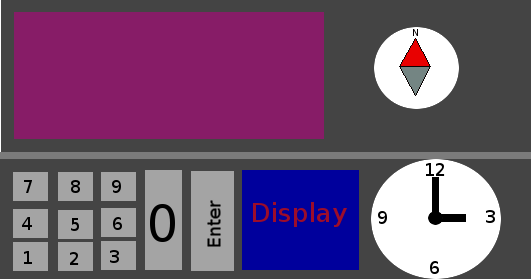
\includegraphics[width=0.8\textwidth]{images/geraet.png}
		\caption{Multifunktionsnavigationsgerät}
		\label{fig:wwu_logo}
	\end{figure}

\aufgabe{2.3}

Das Multifunktionsnavigationsgerät (kurz: MFNG) kombiniert mehrere sinnvolle Bestandteile in ein Gerät. Es ist klein und handlich und kann daher problemlos mitgenommen werden. Das MFNG enthält eine kleine Speicherzelle, die für das Speichern von Daten keinen Strom benötigt. Ferner gibt es eine kleine münzförmige Batterie, die mehrere Jahre im Normalbetrieb hält und leicht austauschbar ist.

Desweiteren gibt es ein Solarpanel, welches im aufgeklappten Zustand das Gerät mit Strom versorgt, wenn die Sonne scheint. Der eingebaute Kompass erlaubt das Ablesen der Himmelsrichtung, in die man gerade fährt. Die Uhr mit eingebautem mechanischem Uhrwerk (initial angetrieben durch die Batterie) erlaubt das Ablesen der Uhrzeit.

Der Standort kann durch Eingabe einiger Parameter in das Gerät errechnet werden. Zu Beginn der Fahrt wird die Uhrzeit, die Zielrichtung und der Sonnenstand (in Relation zur Zielrichtung, ablesbar durch die Augen) mithilfe der Tastatur eingegeben. Möchte man nun später den Standort abfragen, so kann man einen neuen Messpunkt erstellen und die dann aktuellen Daten eintragen. Aus der Zeitdifferenz, dem Unterschied im Sonnenstand und einer zugrundegelegten Heuristik zur durchschnittlichen Kanugeschwindigkeit wird dann die zurückgelegte Entfernung zum Startpunkt ausgegeben.

Eine konkrete Angabe des Standpunktes auf einer Karte ist aufgrund der Beschränkungen nicht umsetzbar. Dies würde GPS, Satelliten und mehr Platz voraussetzen. Ferner wäre ein viel höherer Stromverbrauch anzusetzen, der nicht kompatibel ist mit der mangelnden Verfügbarkeit von Strom.

\end{document}